\subsection*{2.1}
%    1. Build a common-source MOS amplifier as shown below using BS170 transistor.
%Element values: R1 = R2 = 100 k, R3 = R4 = 470 , RL = 1 k, C1 = 1 µF, C2 = 100 µF,
%C3 = 10 µF. Use VDD = 15 V.

    \begin{figure}[h!]
        \centering
        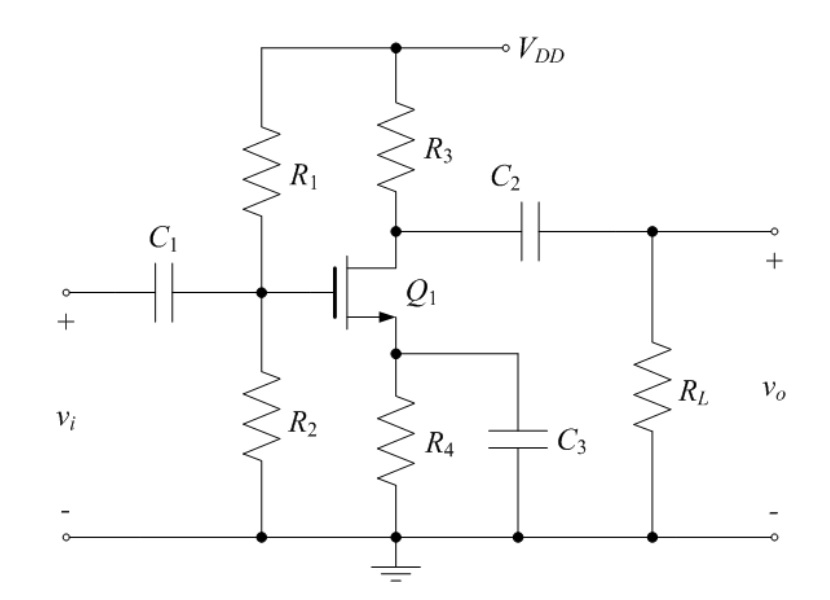
\includegraphics[width=6cm]{circuit_task_2.jpg}
        \captionof{figure}{Circuit built in task 2}
    \end{figure}

\subsection*{2.2}

%2. Use Bode Analyzer to measure the AC characteristic of the amplifier in the frequency
%range 10 Hz to 50 kHz. Use 10 steps per decade and input signal amplitude of 50 mV.
%Find the lower 3dB frequency of the circuit.


\subsection*{2.3}
%3. Determine the following parameters of the circuit (at the frequency 1 kHz): voltage gain,
%input resistance, output resistance. Input signal amplitude should be small, e.g., 50 mV.
%Observe and store the input and output signal waveforms using oscilloscope.
	\begin{figure}[h!]
	    \centering
	    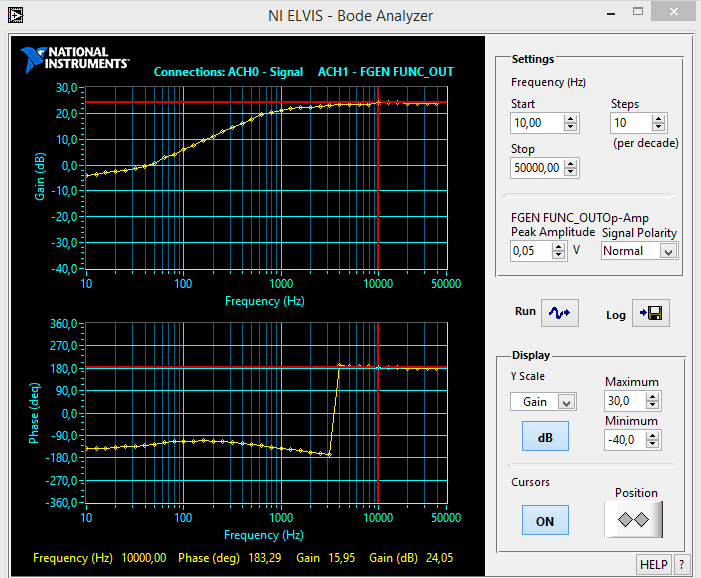
\includegraphics[width=6cm]{Task2.png}
	    \captionof{figure}{Bode analysis of the circuit in figure X }
	\end{figure}

	Figure X shows the Bode Analyzer of circuit in figure X. The cursor shows the midband gain of the circuit.

	$$ A_{M} = 24.05 dB $$ 

\pagebreak
    \begin{figure}[h]
        \centering
        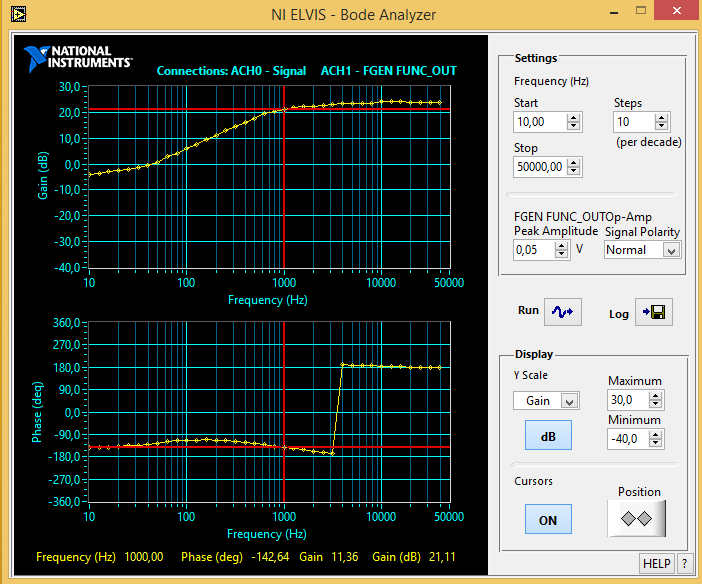
\includegraphics[width=6cm]{Task2-2-1.png}
        \captionof{figure}{Bode analysis of the circuit in figure X}
    \end{figure}

	To find the lower 3dB frequency by finding the 3dB drop to the left from the midband gain 	as seen in figure X.

	$$ f_{L} = 1 \ k Hz $$

    \begin{figure}[h!]
        \centering
        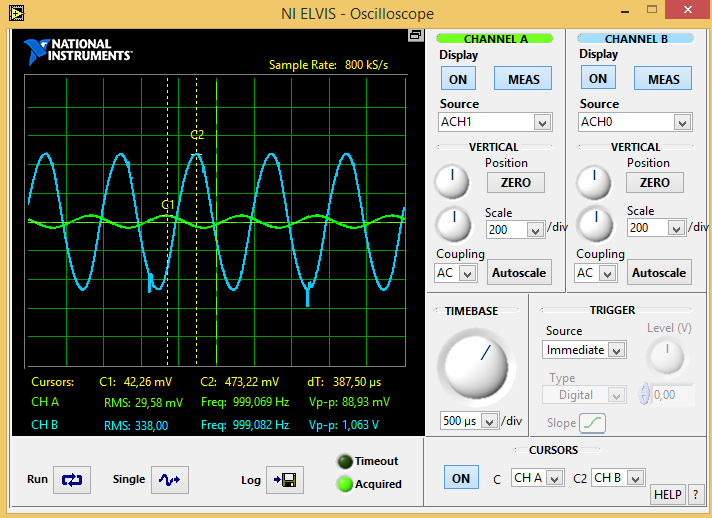
\includegraphics[width=6cm]{Task2-3.png}
        \captionof{figure}{Oscilloscope plot of the circuit in figure X without $R_{s}$}
    \end{figure}

	Figure X shows the Oscilloscope plot of the circuit in figure X. The green wave is the input voltage and the blue wave is the output voltage. By taking the amplitude of blue wave and dividing by amplitude of the green wave gives the midband gain.

	$$ A_{M1} = \frac{473.22 mV}{42.26 mV} = 11.19 \frac{V}{V} $$

\pagebreak

    \begin{figure}[h!]
        \centering
        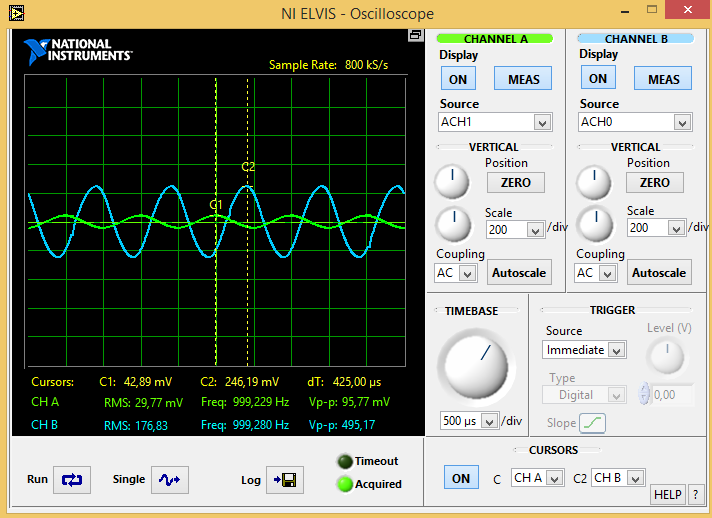
\includegraphics[width=6cm]{Task2-3-Rin.png}
        \captionof{figure}{Oscilloscope plot of the circuit in figure X with $R_s$}
    \end{figure}

	Figure X shows the oscilloscope plot of the circuit in figure X with $R_{s}$. By adding $R_{s}$ to circuit and finding the midband gain of the circuit from the amplitude of the waves in figure X.

	$$ A_{M2} = \frac{245.19 mV}{42.89 mV} = 5.72 $$

	By using the midband gain from circuit without $R_{s}$ and with $R_{s}$. The formula for midband gain with $R_{s}$ would be:  

	$$A_{M2} = A_{M1} \cdot \frac{R_{in}}{R_{in} + R_{s}} \rightarrow R_{in} = \frac{R_{s}}{\frac{A_{M1}}{A_{M2}}-1}  $$

	$$  R_{in} = \frac{46.4 k \Omega }{\frac{11.19}{5.72}-1} = 48.52 k \Omega$$ 

	\begin{figure}[h!]
        \centering
        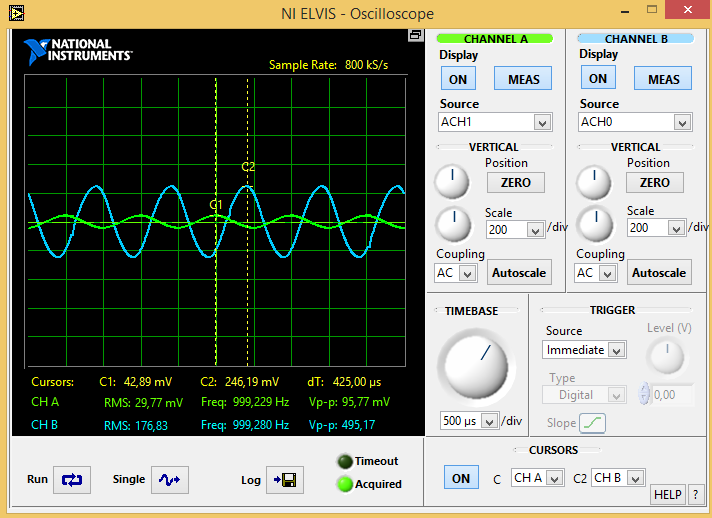
\includegraphics[width=6cm]{Task2-3-Rin.png}
        \captionof{figure}{Oscilloscope plot of the circuit in figure X without $R_L$}
    \end{figure}

	Figure X shows the Osxilloscope plot of the circuit in figure X without $R_{L}$. By removing the load resistor and finding the midband gain from the amplitude of the waves in figure X.


	$$ A_{M3} = \frac{681.05 mV}{42,29 mV} = 16.1 \frac{V}{V} $$

	By using the midband gain from the circuit with $R_{L}$ and without $R_{L}$. The formula for midband gain without $R_{L}$ would be:


	$$ A_{M3} = A_{M1} \cdot \frac{R_{L}}{R_{L} + R_{out}} \rightarrow R_{out} = R_{L} \cdot (\frac{A_{3}}{A_{1}}-1) = 460.72 \frac{V}{V}$$






\subsection*{2.4}
% 4. Using the transistor parameters obtained in Task 1, determine the values of gain,
%input/output resistance and the lower 3dB frequency theoretically compare them to the
%values obtained experimentally.